\section{Introduction}

\begin{wrapfigure}{r}{.4\columnwidth}
\vspace{-5mm}
\centering
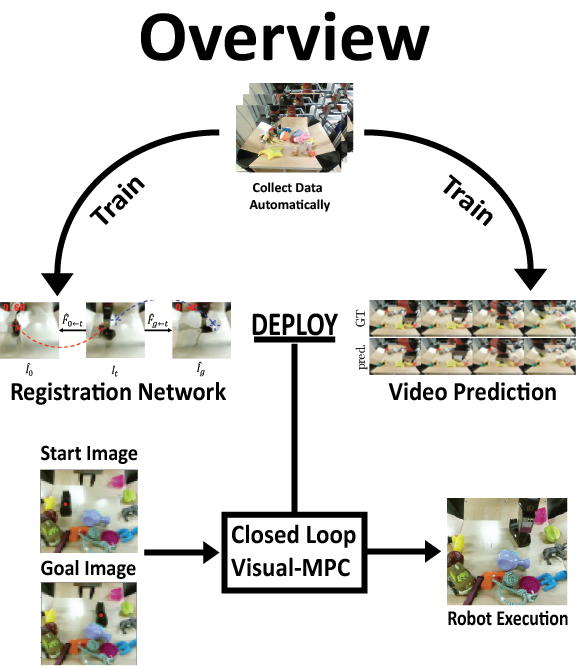
\includegraphics[width=0.4\columnwidth,trim={3.2mm 0 0 0},clip]{images/new_overview}
\caption{\small{Ground truth and predictions from the model (only every 4 frames are shown). These examples show grasping, pushing, and simultaneous grasping and dragging. }}
\label{fig:video_prediction}
\vspace{-0.2in}
\end{wrapfigure}

Humans have the ability to learn complex skills such as manipulating objects through millions of interactions with their environment during their lifetime.
These interactions enable us to acquire a general understanding of the physical world and, notably, do not require significant supervision beyond observation of one's own actions and their consequences. Hence, self-supervised learning through prediction is an appealing direction of research as it enables intelligent systems to leverage and learn from massive amounts of unlabeled raw data to autonomously acquire general skills. Yet, self-supervised learning systems using predictive models of sensory inputs present a number of challenges: planning needs to account for imperfections in the predictive model and the robot needs a grounded mechanism for evaluating predicted futures.
How can we enable systems to plan to perform complex tasks from raw sensory observations, even when the predictions are not always accurate?

Prior work on self-supervised robot learning has enabled robots to learn rudimentary, short-term manipulation skills such as grasping~\cite{lerrel,google_handeye}, singulation~\cite{princeton_pushgrasp}, pushing~\cite{foresight,sna}, poking~\cite{pulkit}, and other arm motions~\cite{se3_control}. The question that we are concerned with in this work is: can self-supervised predictive models of raw visual observations be used to perform more complex and realistic tasks, especially tasks that are temporally extended? 
%, closed-loop control of multiple forms of behavior and goals through self-supervision remains an open problem.
%Prior work has demonstrated that video prediction can be used for rudimentary, short-term robotic manipulation tasks in the real world, such as pushing objects~\cite{}. The question we are concerned with in this work is: can direct video prediction be used to perform more complex and realistic tasks, especially tasks that are temporally extended? 
While this might seem exceedingly challenging due to the difficulty of long-term prediction of images, we make use of the well-known principle of model-predictive control (MPC) that allows targeting long-terms goals with a relatively short prediction horizons. To allow effective replanning, we need a planning objective that allows the robot to reliably make progress towards the goal.
%that is optimized by a short-horizon planner allowing to reliably make progress towards the goal. 

%While this might seem exceedingly challenging due to the difficulty of long-term prediction of images, we make the following observation: that make it feasible to perform relatively long-horizon tasks. First, we observe that short-horizon planning can still give us a good indication of the potential for a plan to achieve a long-term goal, if provided with the right cost function. This fact has been known for decades, and is the basis for model-predictive control: iterative short-horizon replanning that aims to achieve long-term goals. Yet, maintaining an accurate estimate of the cost function throughout planning is crucial.
We propose a cost function based on image-to-image registration, which we demonstrate can itself be learned without any human supervision using the same exact dataset as the one used to train the predictive model. The key element that enables our method to perform long-horizon tasks is that, using our cost function, the robot can always evaluate the distance to the goal, allowing it to continuously retry, so that even flawed predictions allow for an eventual successful execution. 



%Closed-loop control allows the robot to be persistent, correcting for mistakes caused by inevitable model inaccuracies and continuously retrying until it succeeds.
%Further, learning models that can be used to plan multiple types of behaviors is critical for learning general-purpose control.
%%SL.06.12: there are two ideas above: (1) learning models that can be used for various tasks is important for general-purpose control (2) retrying is a good idea; these ideas are kind of stuck together awkwardly a bit, can we push them apart so that one builds on the other?
%In this work, we aim to develop a learning system that interacts with the environment autonomously, building a model that can be used to plan a variety of motions, including pushing, grasping, and placing, while enabling the agent to continuously try and retry the task until it succeeds.
%%SL.06.12: the title says something about being precise -- where does that come in?

%A robot equipped with action-conditioned predictive models of future observations has some understanding of the physical world and how it changes as a consequence of its actions. Such model could then be used by the robot to plan multiple types of behaviors for general-purpose control. These models can be learned through self-supervision, whereby the robot interacts with the environment through random actions while observing through its sensors. In our work, we use a video prediction model that predicts future frames conditioned on actions and past frames.

%%AL.06.13: I think we need two paragraphs that contains the following information:
% Paragraph on self-supervised learning. Massive amounts of self-supervised data. Action-conditioned video prediction model that predicts future frames by implicitly transforming pixels from previous frames via image-space flow fields. These flows can be used for planning given a designated pixel position in the first frame and goal pixel position in the goal frame (say how it's done). Forward models can deviate from the truth very quickly due to compounding errors. Naturally, replanning (MPC). However, we don't have good cost functions since we have lost designed pixel position in the new first frame. Solution?
% Paragraph on registration. Track designed pixel position. Allows for more precise retrying. Registration registers to both first and goal frames, so can be accurate near beginning and end of trajectory.


%%SL.04.20: I would recommend reading through this carefully and noting the key points that we need to touch on in an introduction: https://cs.stanford.edu/people/widom/paper-writing.html


We demonstrate our method on the task of maneuvering unknown objects in a table-top setting using a robot manipulator. To autonomously learn to perform manipulation skills with high-fidelity, tasks need to be specified in way that allows for precision and retrying. We specify a goal by providing an image of the desired configuration along with user-annotated positions of the objects of interest\footnote{This also allows the user to specify distractor objects that can be ignored in the goal image}. This provides a straight-forward and grounded mechanism for a human to provide a goal in the observation space of the robot.
Building upon prior methods that use self-supervised predictive models for control~\cite{foresight,sna,se3_control}, we develop a method that can plan actions with a video prediction model to achieve the desired state specified in the goal image.
%%SL.06.12: I feel like maybe we should explicitly say that our method builds on prior work (foresight, sna), since in this case the contribution might actually be easier to understand if we explicitly frame it in terms of prior work. It might open us up to accusations that the work is incremental, but I think that is less bad than a lack of clarity about the nature of the contribution

The main contribution of this work is a method for computing the planning cost based on image-to-image registration by using a learned registration model to find correspondences  between the current image and both the goal image and the initial image.
%We train a deep convolutional network to find these correspondences by learning an image-to-image warping function in a self-supervised manner. 
This allows closed-loop control, enabling the robot to persistently attempt the task until completion. In contrast to the short-horizon pushing skills and arm motions demonstrated in prior work~\cite{foresight,sna,se3_control}, we show that our video prediction model can be used to perform longer-term manipulations, autonomously choosing when to push or to  pick objects, and, when provided enough time, accomplish tasks significantly more consistently.
In addition we show that a joint pushing and grasping-policy can be emerge from pure self-supervised learning. Furthermore by using with two separate views for video-prediction and task specification, 3D-tasks manipulation tasks can be solved.

%Compared to prior work on self-supervised learning and hand-engineered tracking modules, we find that our approach is able to perform a variety of object manipulation tasks and, when provided enough time, achieve tasks significantly more consistently.

%%SL.06.12: Some high level comments on the introduction: Currently, it doesn't really talk about grasping -- it just abstractly says that there are multiple skills, but not what those skills are. Can we elaborate on this point a little bit? I think the current intro is definitely better, but we should try to do a better job of coming up with the story. I think we should make sure we touch on the following points/questions:
%Prior work has demonstrated that video prediction can be used for rudimentary, short-term robotic manipulation tasks in the real world, such as pushing objects~\cite{}. The question we are concerned with in this work is: can direct video prediction be used to perform more complex and realistic tasks, especially tasks that are temporally extended? While this might seem exceedingly challenging due to the difficulty of long-term prediction of images, we make the following observations that make it feasible to perform relatively long-horizon tasks. First, we observe that short-horizon planning can still give us a good indication of the potential for a plan to achieve a long-term goal, if provided with the right cost function. This fact has been known for decades, and is the basis for model-predictive control: iterative short-horizon replanning that aims to achieve long-term goals. For video prediction, we propose a cost function based on image registration, which we demonstrate can itself be learned without any human supervision using the same exact dataset as the one used to train the predictive model. The second idea that enables our method to perform long-horizon tasks is that, if the robot can always evaluate the goal, it can continuously retry, so that even flawed predictions allow for an eventual successful execution. We use the same learned registration model to enable this retrying behavior.
%
%In contrast to the short-horizon pushing skills demonstrated in prior work~\cite{}, we show that our video prediction model can be used to perform longer-term manipulations and automatically choose to push and pick objects, acquiring rudimentary grasping behaviors entirely via video prediction.

%this registration network learns a function that transforms images from arbitrary timesteps along a video to match frames from other timesteps. 







